\chapter{Expression of collapsin response mediator protein 4 in the presence of altered retinogeniculate input}
\textbf{Abstract}\\
\textbf{Collapsin response mediator protein 4 (CRMP4) is expressed in the interlaminar zones of the developing lateral geniculate nucleus (LGN).  CRMP4 expression in the LGN is highest during a developmental epoch in which eye specific segregation of retinal ganglion cells has taken place, but the final cytoarchitecture of the nucleus has not yet been established. The onset of CRMP4 expression is coincident with the formation of cell sparse interlaminar zones in the LGN and CRMP4 expression declines after the cytoarchitecture of the nucleus has reached a mature state.  Here, I manipulate the normal development of LGN cytoarchitecture through binocular and monocular enucleation and disruption of cholinergic retinal waves with epibatidine.  CRMP4 expression in the presence of aberrant LGN cytoarchitecture is then assayed using immunohistochemistry.  Enucleation alters the laminar boundaries and expression of CRMP4 in the LGN in a manner consistent with the altered distribution of retinal axons.  Blockade of cholinergic retinal waves with epibatidine in the first ten days of life induces aberrant eye specific segregation of retinal ganglion cell afferents as well as abolishes both the formation of normal cell sparse interlaminar zones and CRMP4 expression.  Taken Together, the expression pattern of CRMP4 in enucleate and epibatidine treated LGNs demonstrates that CRMP4 expression is driven by the morphology of cell sparse interlaminar zones and not by eye specific segregation.}

\section{Introduction}
In the normal ferret, retinal afferents from both eyes are intermingled in the LGN at birth and become well segregated by P10 (Linden et al., 1981b).  It is clear that the proper segregation of retinal afferents is dependent on the activity of the retinas themselves and is abolished by activity block in the retina (Penn et al., 1998b; Huberman et al., 2002).  At birth, endogenous activity in the retina takes the form of traveling waves of cholinergic activity initiated in starburst amacrine cells (Feller et al., 1996; Penn et al., 1998b; Feller, 1999). This pattern of activity persists in the retina for the first two weeks of postnatal life.   When retinal waves are blocked for the first ten days of life using epibatidine, a selective cholinergic blocker, the normal segregation of eye specific afferents in the LGN does not occur and an overlapping distribution of afferents results (Penn et al., 1998b).  If recovery is allowed after the initial blockade of retinal waves, segregation is achieved, but the retinal afferents fail to project into the correct LGN laminae.  Further, the LGN fails to develop the normal cytoarchitecture associated with mature LGNs (Huberman et al., 2002).  

The normal distribution of retinal afferents and organization of the cytoarchitecture in the LGN can also be manipulated by enucleation at birth.  Binocular enucleation at birth degrades all retinal afferents in the LGN and eliminates lamination (Brunso-Bechtold and Casagrande, 1981).  Monocular enucleation at birth causes the retinal afferents of the spared eye to gradually expand into the normal territory of the enucleated eye after the initial formation of the nucleus.  By the third postnatal week, the afferents of the spared eye occupy the full volume of the nucleus (Guillery et al., 1985). 

In the first part of this chapter, I confirm the above results from studies of epibatidine treatment as well as a report of epibatidine treatment shifting the ipsilateral projection along the medial to lateral axis of the LGN (Padmanabhan, 2008).  Following my characterization of the impact of epibatidine on the projection pattern of retinal afferents in the LGN, I demonstrate that epibatidine treatment abolishes the normal pattern of CRMP4 expression in the LGN reported in chapter 3.  In the second part of this chapter, I report the impact of binocular and monocular enucleation on the normal pattern of CRMP4 expression in the LGN.

\section{Materials and methods}
\subsection{Tissue preparation}
All ferret and mouse experiments were conducted in accordance with protocols approved by the Carnegie Mellon University institutional animal care and use committee.� Seventeen ( 5 monocular enucleate, 4 binocular enucleate, 5 epibatidine treated, 3 saline controls) black sable ferrets (Mustela putorius furo) between the ages of postnatal day 0 (P0) and adulthood were sacrificed and perfused for histology following either enucleation or epibatidine treatment (see 4.2.2 and 4.2.3) and recovery.  Ferrets were sacrificed with an overdose of sodium pentobarbital (250mg/kg) then perfused transcardially with 0.9\% NaCl, 4\% paraformaldehyde, and 4\% parafomaldehyde with 30\% sucrose, all  in .1M phosphate buffer.� Tissue was post-fixed for a minimum of 24 hours before sectioning.  Horizontal LGN sections were made from one LGN per animal at 50$\mu$m using a freezing microtome.

\subsection{Monocular and binocular enucleation}
Ferret� enucleations were performed using hypothermia anesthesia and sterile technique on P0 as described previously (Crowley and Katz, 1999).� Enucleated animals developed normally until they were processed as above.� Two days before monocular enucleates were sacrificed, the spared eye was injected with cholera toxin $\beta$-subunit conjugated to alexa-488 under isoflurane anesthesia in order to visualize the organization of the retinogeniculate projection.

\subsection{Intravitreal application of epibatidine}
\emph{In vivo} intravitreal application of epibatidine was carried out as previously described (Huberman et al., 2002).  Briefly, ferrets were anesthetized with inhaled isoflurane and 1-2$\mu$l of epibatidine (1mM in sterile saline) or sterile saline was injected into the vitreous humor of each eye every 48 hours from P1 to P9.  The animals were allowed to recover until P28 and injection of cholera toxin $\beta$-subunit conjugated to alexa-555 in one eye and cholera toxin $\beta$-subunit conjugated to alexa-647 in the other as above.  Epibatidine or saline control animals were sacrificed at P30 and prepared for histology as described above.

\subsection{Immunohistochemistry}
Immunohistochemical stains against CRMP4 were carried out as described in 3.2.3.

\subsection{Myelin staining}
Myelin staining was carried out as described in 3.2.5.

\subsection{Image analysis for epibatidine disruption of retinothalamic projections}
All images were acquired and converted to binary images using maximum correlation thresholding (Padmanabhan et al., 2010).  Percent overlap values for the contralateral and ipsilateral retinothalamic projection were calculated by counting the number of yellow pixels in binarized images vs. the total number of pixels in the projection domain.  For the calculation of mediolateral and rostrocaudal position, the weighted centroid of the ipsilateral projection was  calculated and expressed as a normalized position along the two axes of the nucleus.  For perimeter to area calculations, a single pixel edge was calculated around all projection domains.  This edge was calculated by uniformly shrinking the boundaries of binarized projection domains and subtracting this shrunk version from the original binarized domain leaving a single pixel edge at the projection boundaries.  The number of pixels in the edge regions was compared to the total number of pixels in the projection domains themselves for perimeter to area measures. All epibatidine morphological measures are same as used previously for the same analysis in our lab (Padmanabhan, 2008).

\subsection{Image analysis for laminar expression of CRMP4 and Myelin}
Analysis of CRMP4 and myelin laminar patterns was carried out as described in 3.2.6.

\section{Results}
\subsection{Transient epibatidine block of retinal activity disrupts normal retinal projections, normal cytoarchitecture, and normal CRMP4 expression in the LGN}
Retinal activity was blocked using epibatidine for the first 10 days of postnatal life followed by recovery until P30.  The resultant projection pattern and laminar organization of the LGN mirrored what has been previously reported (Huberman et al., 2002; Padmanabhan, 2008).  In normal P30 ferrets there is a rather stereotyped retinothalamic connection and lamination pattern consisting of a single major projection of ipsilateral retinal ganglion cells to the A1 lamina and and minor projection in the C1 lamina of the LGN (Linden et al., 1981b).  Saline controls in the present study exhibit this typical morphology (figure 4.1a).  Epibatidine treated animals did not show the normal projection and lamination pattern and were instead characterized by multiple major ipsilateral projections (figure 4.1b,c).  In order to determine the degree to which the ipsilateral projection was scattered in epibatidine animals, I quantified the number of ipsilateral projections, ipsilateral projection surface area/volume ratio, and the contralateral surface area/volume ratio.  There were significantly more ipsilateral projections to the LGNs of epibatidine animals (figure 4.1c, saline = 1.0$\pm$0.0 patches, epibatidine = 3.2$\pm$0.2 patches, P $<$ .001, student�s t-test).  There was also a significantly higher surface area/volume ratio of the ipsilateral projection in epibatidine animals (figure 4.1d, saline = 0.037$\pm$0.005, epibatidine = 0.070$\pm$0.006, p = 0.004, student�s t-test), but not of the contralateral projection (figure 4.1e, saline =  0.030$\pm$0.005, epibatidine = 0.028$\pm$0.004, p = .787, student�s t-test).  Although the normal pattern of retinothalamic projections to the LGN was altered in these animals, there was no difference in the total volume of the contralateral (figure 4.2a, saline = 81.84$\pm$2.83\%, epibatidine =  86.48$\pm$2.00\%, p = 0.12, student�s t-test) and ipsilateral (figure 4.2b, saline = 18.67$\pm$3.50\%, epibatidine =  14.53$\pm$2.26\%, p = 0.22, student�s t-test) projections between saline controls and epibatidine treated animals.  Further, the segregation between ipsilateral and contralateral projections was unchanged in epibatidine animals (figure 4.2c, saline percent overlap = 0.64$\pm$0.45\%, epibatidine percent overlap = 1.02$\pm$0.50\%, p = .56, student�s t-test).  In addition to the above measures, I quantified the mean rostrocaudal and mediolateral position of the ipsilateral projection in epibatidine treated animals (figure 4.3).  There was no difference in the rostrocaudal position of the ipsilateral projection into the LGN (figure 4.3b, saline = 0.71$\pm$0.04, epibatidine = 0.75$\pm$0.04, p = 0.43, student�s t-test), but there was a significant medial shift epibatidine treated animals (figure 4.3c, saline = 0.50$\pm$0.04, 0.31$\pm$0.03, P $<$ 0.01, student�s t-test).  All morphological parameters measured above are in agreement with previous studies of epibatidine treated animals in our lab (Padmanabhan, 2008).

In addition to the observed disruption in retinothalamic projection morphology, epibatidine treatment disrupts the normal cytoarchitecture of the LGN.  In the normal P30 LGN, the laminae of the nucleus are separated by cell sparse interlaminar zones along with ON/OFF cell sparse sublaminar boundaries in the A and A1 laminae (Linden et al., 1981b; Stryker and Zahs, 1983).  These cell sparse zones are abolished in my epibatidine treated animals (figure 4.4).  The lack of cell sparse interlaminar zones in the epibatidine treated P30 ferret is consistent with previous work by Huberman et al (Huberman et al., 2002).  

To assess the extent to which CRMP4 expression is linked to the normal eye specific segregation in the developing LGN, we stained epibatidine treated LGNs for CRMP4 at P30.  Epibatidine treatment decouples eye specific segregation from lamination in the LGN and allows us to study the correlation of CRMP4 expression to the two processes independently (Huberman et al., 2002).  In P30 epibatidine treated animals, the pattern of eye specific projections into the LGN was disrupted compared to normal animals and there was no laminar expression of CRMP4 above background (figure 4.5).  Myelin expression in the LGN of epibatidine treated animals was also disrupted.  In normal animals, there is dense myelin staining both at the PGN/LGN boundary and at interlaminar zones (see figure 3.6).  In epibatidine treated animals, there is very little myelin expression above background at the interlaminar zones and only the LGN/PGN boundary shows significant myelin expression (figure 4.6).

%------------------------------------Chapter 4 results figs 1-----------------------------------------------
\pagebreak
\begin{figure}[htb!]
\begin{center}
\leavevmode
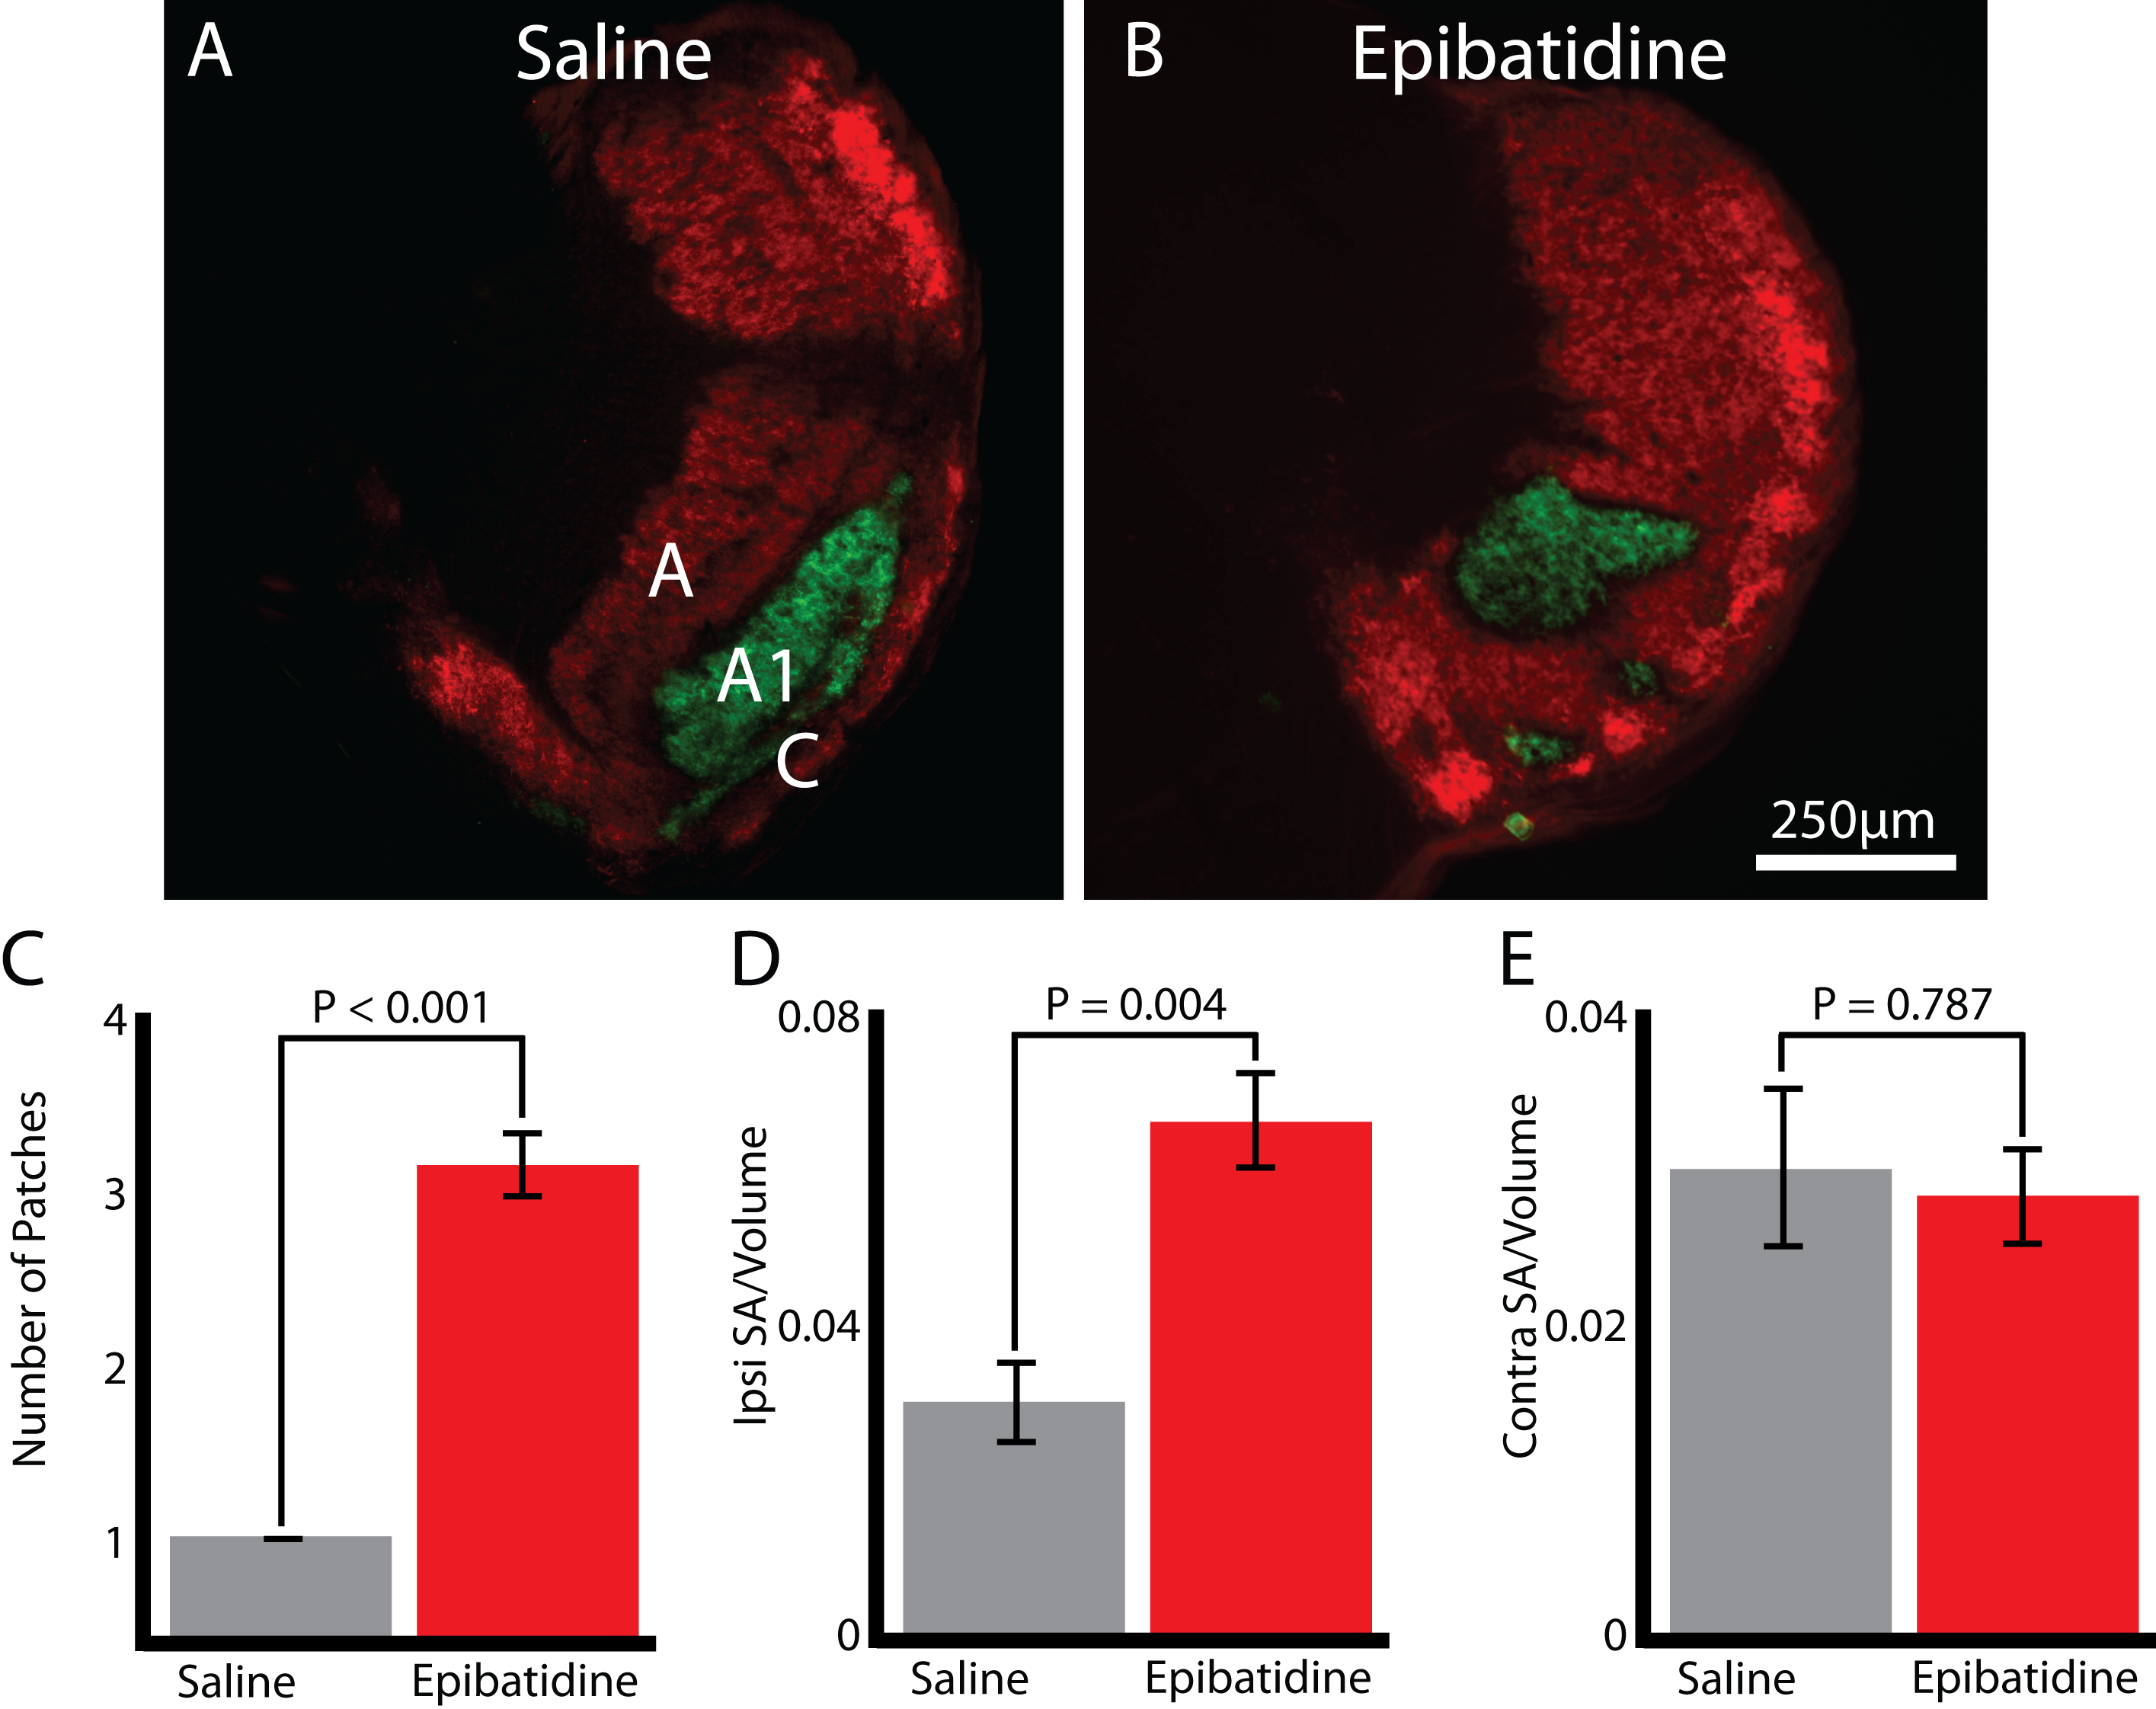
\includegraphics[width=1.0\textwidth]{FigureImages/EpiPatchesQuant.png}
\end{center}
\caption[ Epibatidine treatment alters the pattern of retinothalamic projections into the LGN.]{ Epibatidine treatment alters the pattern of retinothalamic projections into the LGN. A, normal P30 ferret LGN in horizontal section.  contralateral projections (red) display major terminations into the A lamina while major terminations from the ipsilateral retina (green) terminate in the A1 lamina.  Minor projections from both retinas terminate in the C laminae.  B, epibatidine treated ferrets show disrupted retinothalamic projection patterns at P30.  Multiple ipsilateral projections are visible and the contralateral projection is reorganized to fill the space normally occupied by parts of the ipsilateral projection. C, epibatidine treated ferrets display more ipsilateral patches in the LGN than saline controls.  D, epibatidine animals also show smaller ipsilateral projection domains as measured by the surface area/volume of these projections.  E, There is no difference between the surface area/volume measure of the contralateral projection.}
\end{figure}

\pagebreak
\begin{figure}[htb!]
\begin{center}
\leavevmode
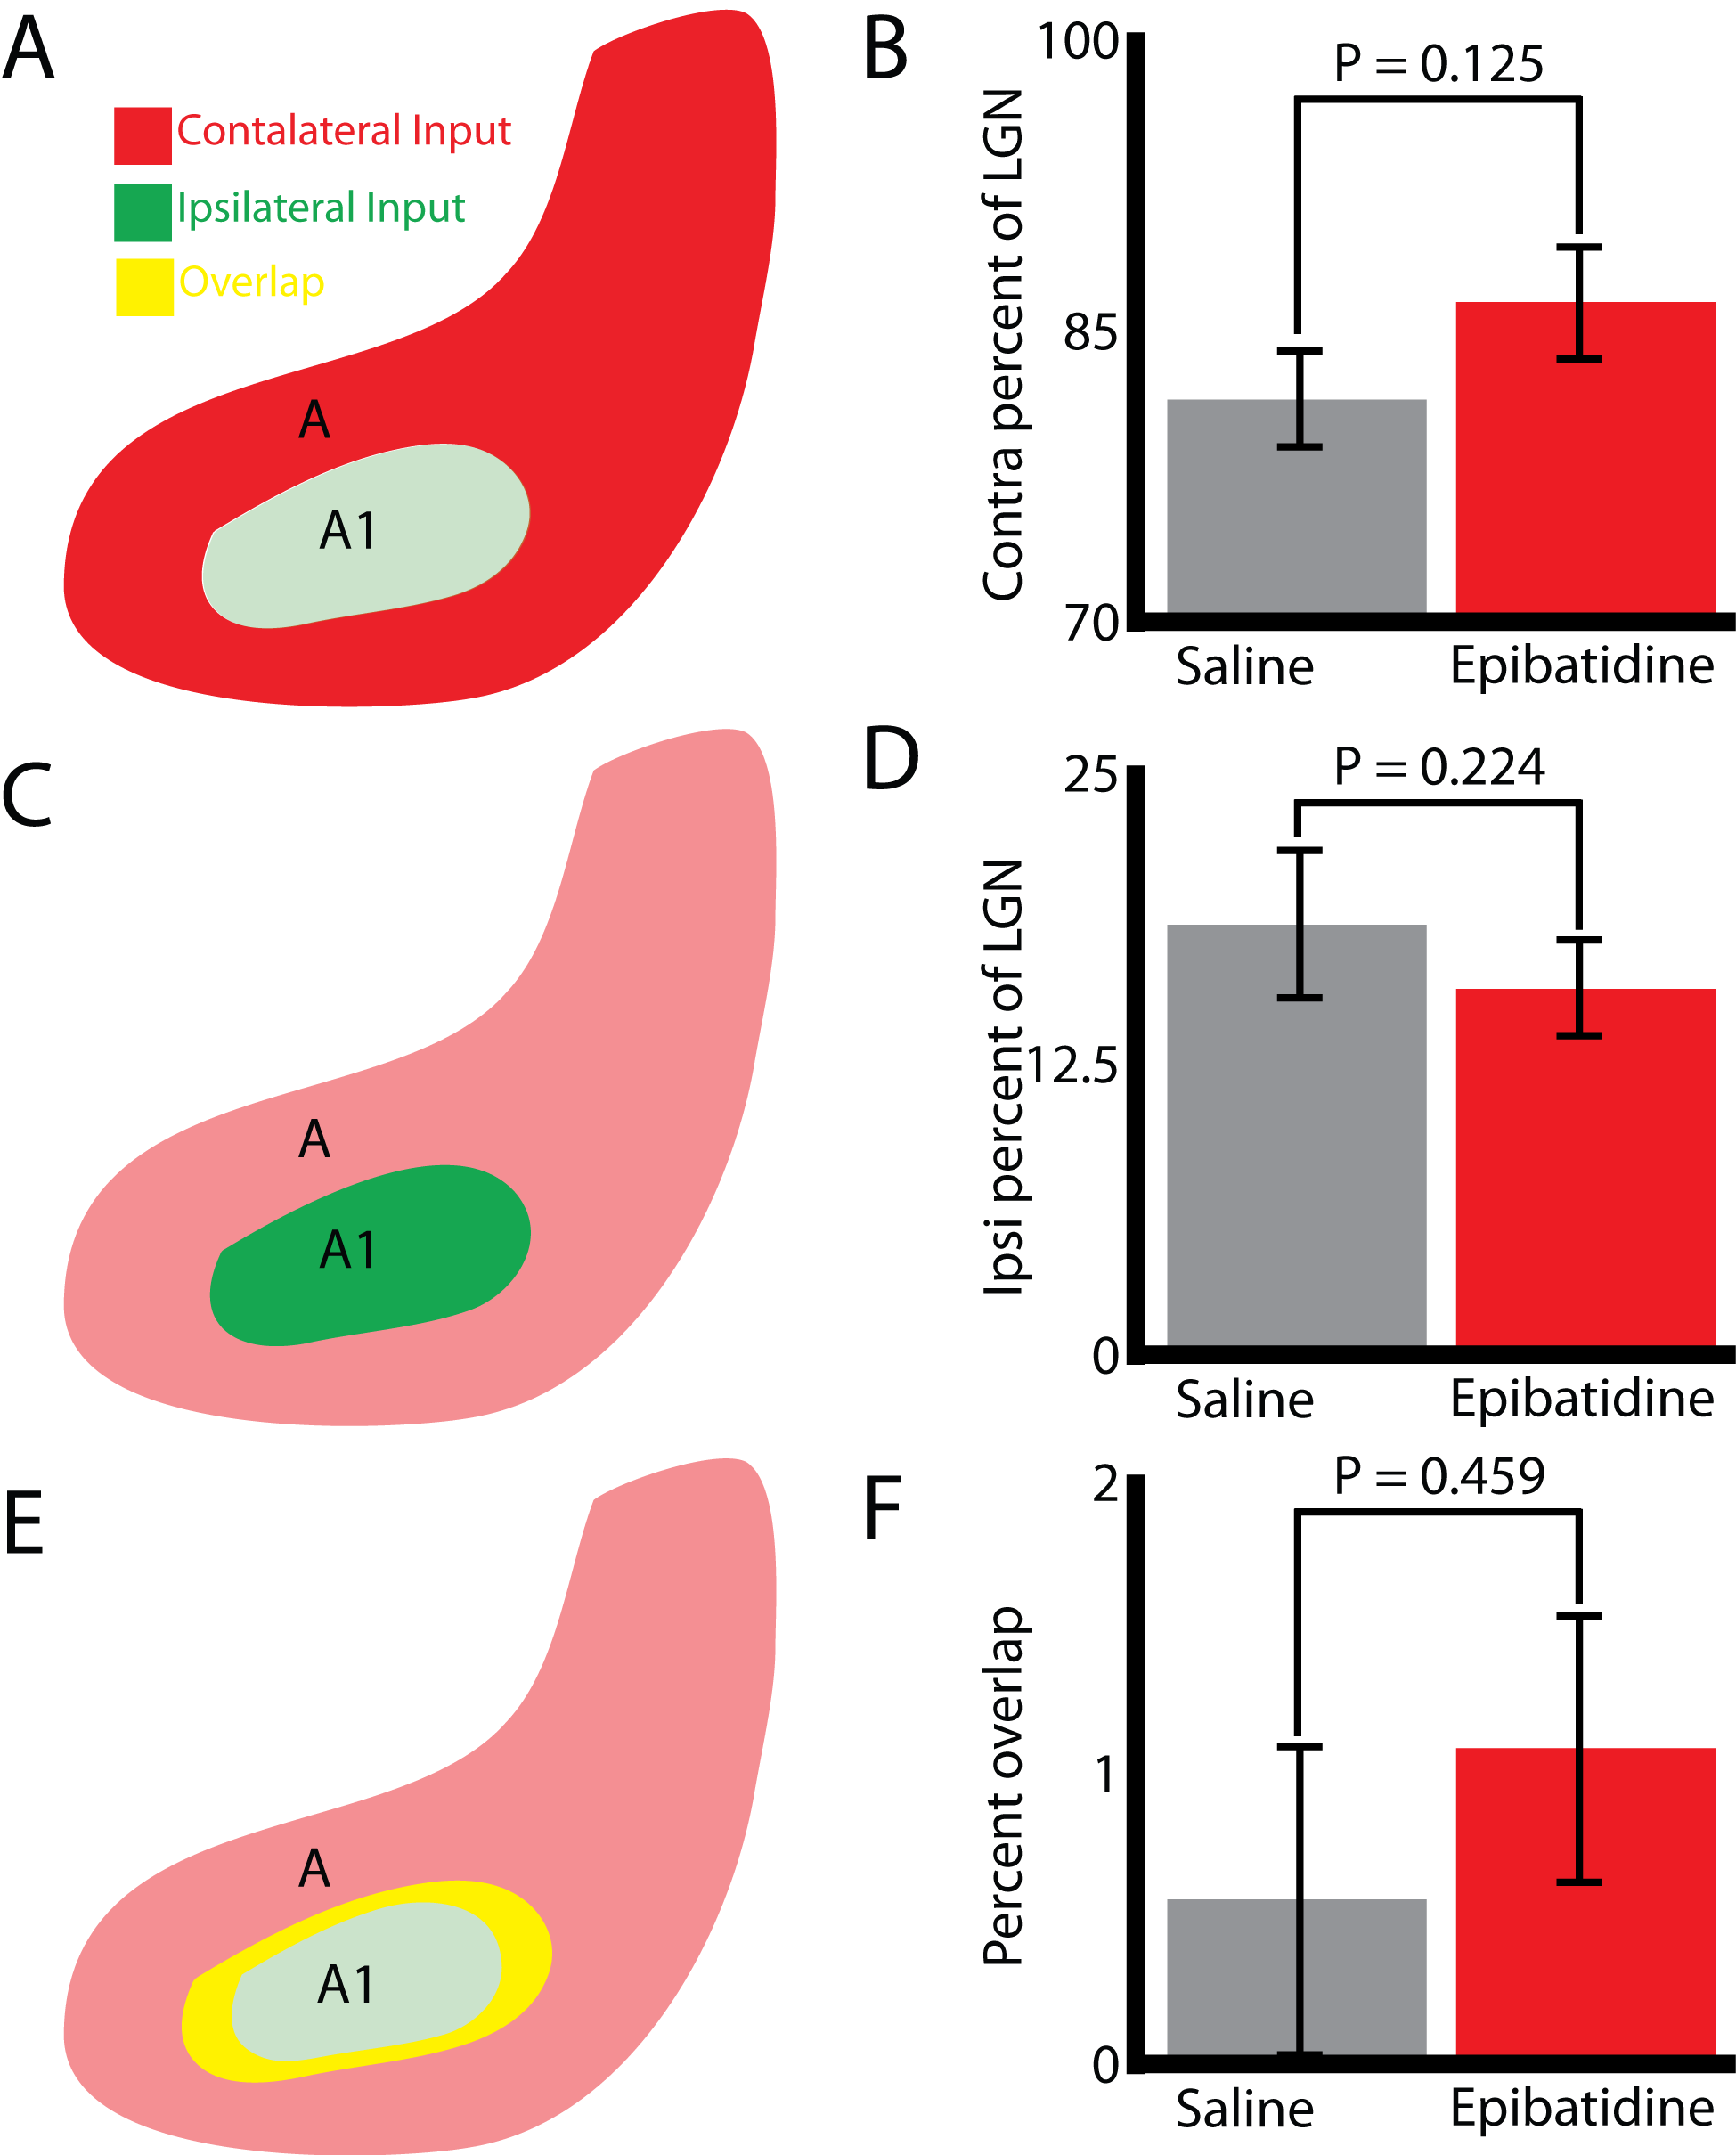
\includegraphics[width=0.8\textwidth]{FigureImages/EpiOverlapQuant.png}
\end{center}
\caption[ Epibatidine treatment does not alter the size or segregation of ipsilateral and contralateral retinothalamic projections to the LGN.]{ Epibatidine treatment does not alter the size or segregation of ipsilateral and contralateral retinothalamic projections to the LGN. A, C, and E, diagrams of the contralateral projection, ipsilateral projection, and overlap between the two, respectively.  B, there is no difference in the percentage of the total LGN volume occupied by the contralateral projection between saline and epibatidine treated animals.  D, there is also no difference in the percentage of the LGN occupied by the ipsilateral projection.  F, the degree of overlap between the ipsilateral and contralateral projections is not altered in epibatidine treated animals.}
\end{figure}

\pagebreak
\begin{figure}[htb!]
\begin{center}
\leavevmode
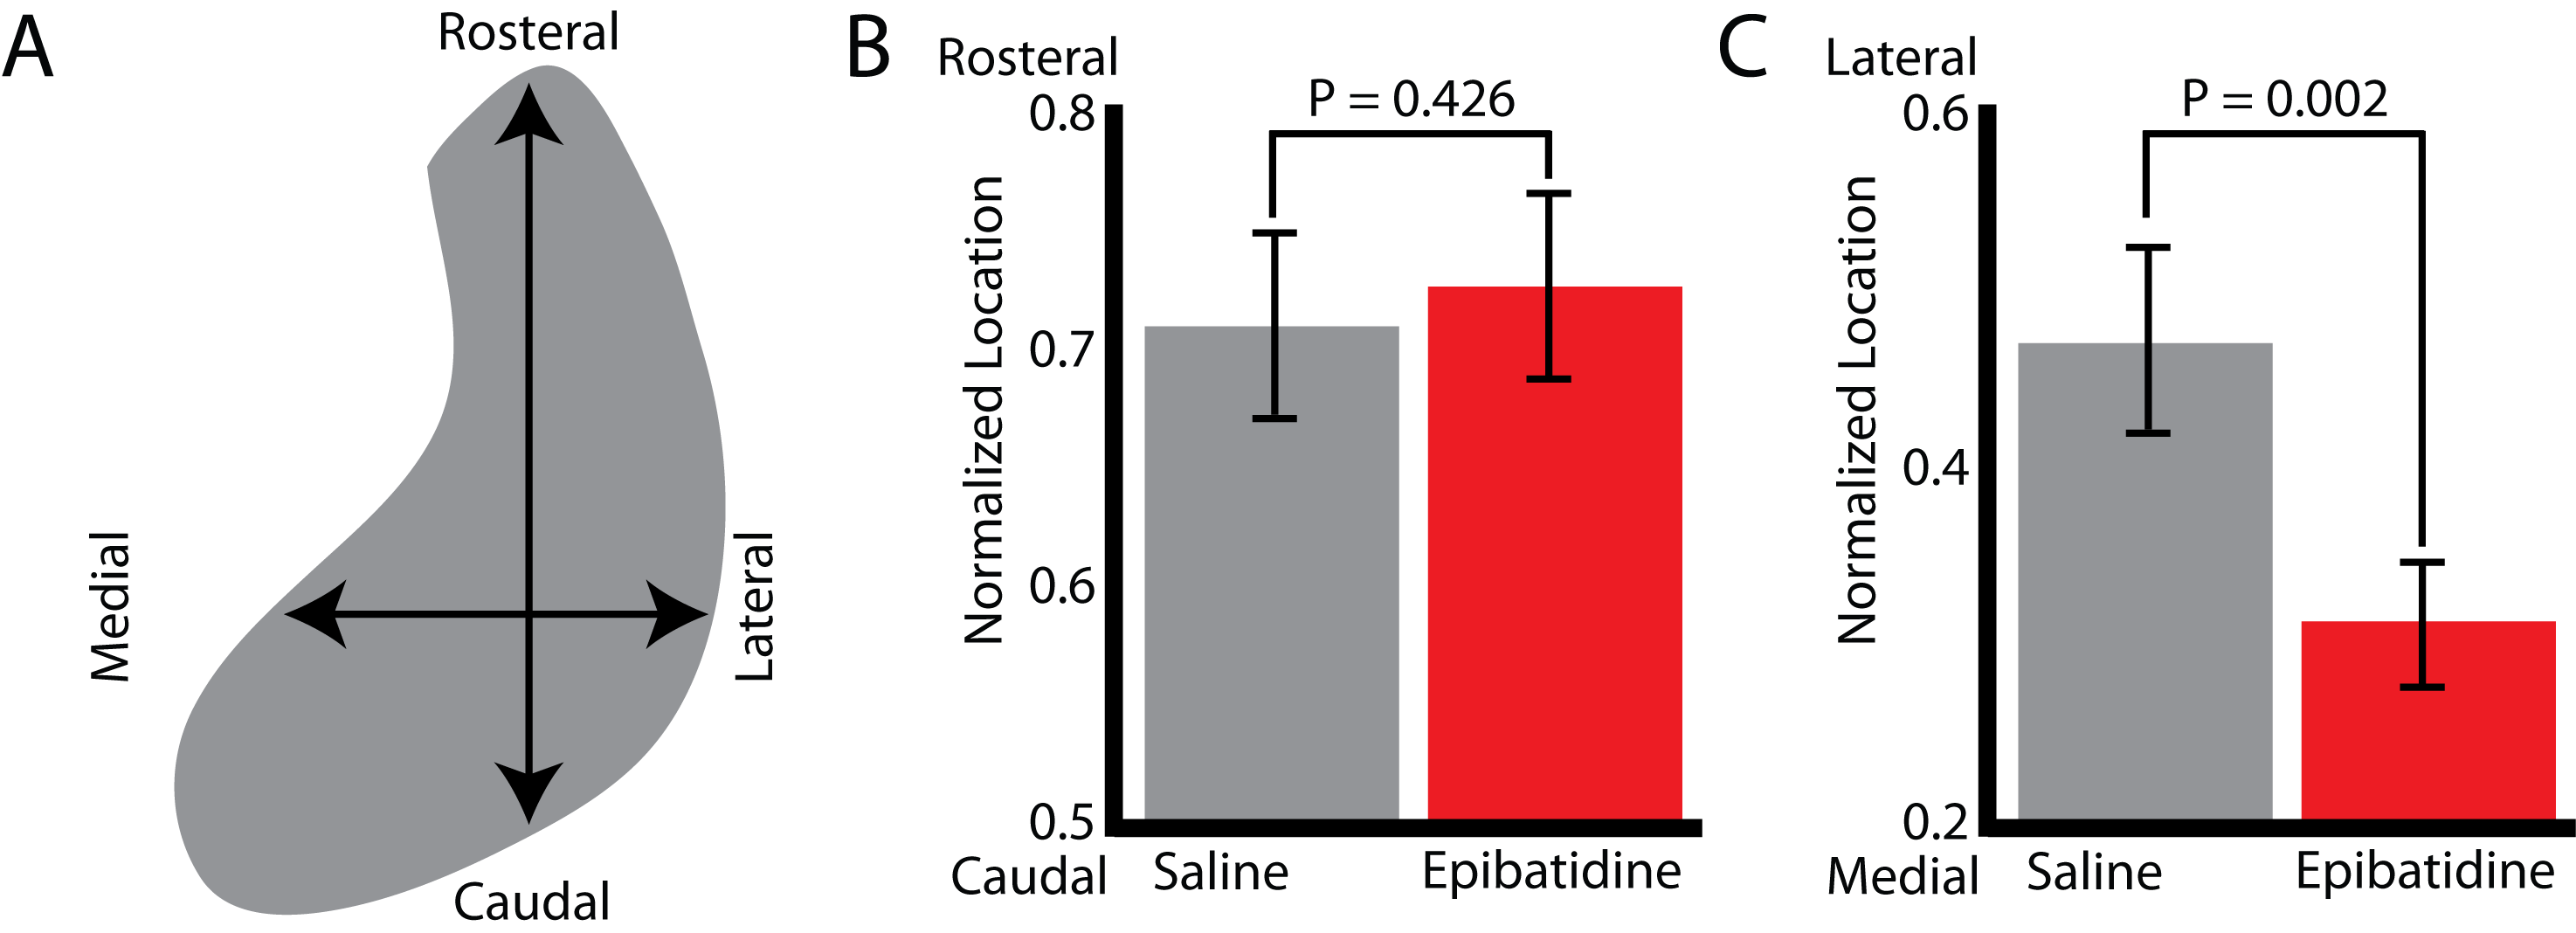
\includegraphics[width=1.0\textwidth]{FigureImages/EpiPositionQuant.png}
\end{center}
\caption[ Epibatidine treatment causes a medial shift in the ipsilateral retinothalamic projection to the LGN.]{Epibatidine treatment causes a medial shift in the ipsilateral retinothalamic projection to the LGN. A, diagram of the position of the rostrocaudal and mediolateral axes in a horizontal section of the ferret LGN.  B, there is no significant shift in the position of ipsilateral projections to the LGN along the rostrocaudal axis under epibatidine treatment.  C, there is a significant medial shift in the position of the ipsilateral projection along the mediolateral axis under epibatidine treatment.}
\end{figure}

\pagebreak
\begin{figure}[htb!]
\begin{center}
\leavevmode
\includegraphics[width=1.0\textwidth]{FigureImages/NisslCTBComparison.png}
\end{center}
\caption[Epibatidine treatment abolishes normal LGN cytoarchitecture.]{Epibatidine treatment abolishes normal LGN cytoarchitecture. A, horizontal slice of  a normal P30 LGN with ipsilateral retinal projections labeled in green and contralateral projections labeled in red.  Clear gaps in the density of projections are visible at the laminar and ON/OFF sublaminar boundaries (white arrows).   B, Nissl stain of an adjacent slice to A.  Cell sparse regions are visible at laminar and ON/OFF sublaminar boundaries (black arrows).  C, larger view of the white box in A.  D, larger view of the red box in B. E, horizontal slice of an epibatidine treated P30 LGN with ipsilateral retinal projections labeled in green and contralateral projections labeled in red.  The organization of the retinothalamic projections is disrupted relative to saline controls.  F, Nissl stain of an adjacent slice to E.  There are no clear cell sparse zones akin to those seen in saline controls.  G and H, larger views of the white and red boxes in E and F, respectively.scale bar = 250 $\mu$m, applies to all}
\end{figure}

\pagebreak
\begin{figure}[htb!]
\begin{center}
\leavevmode
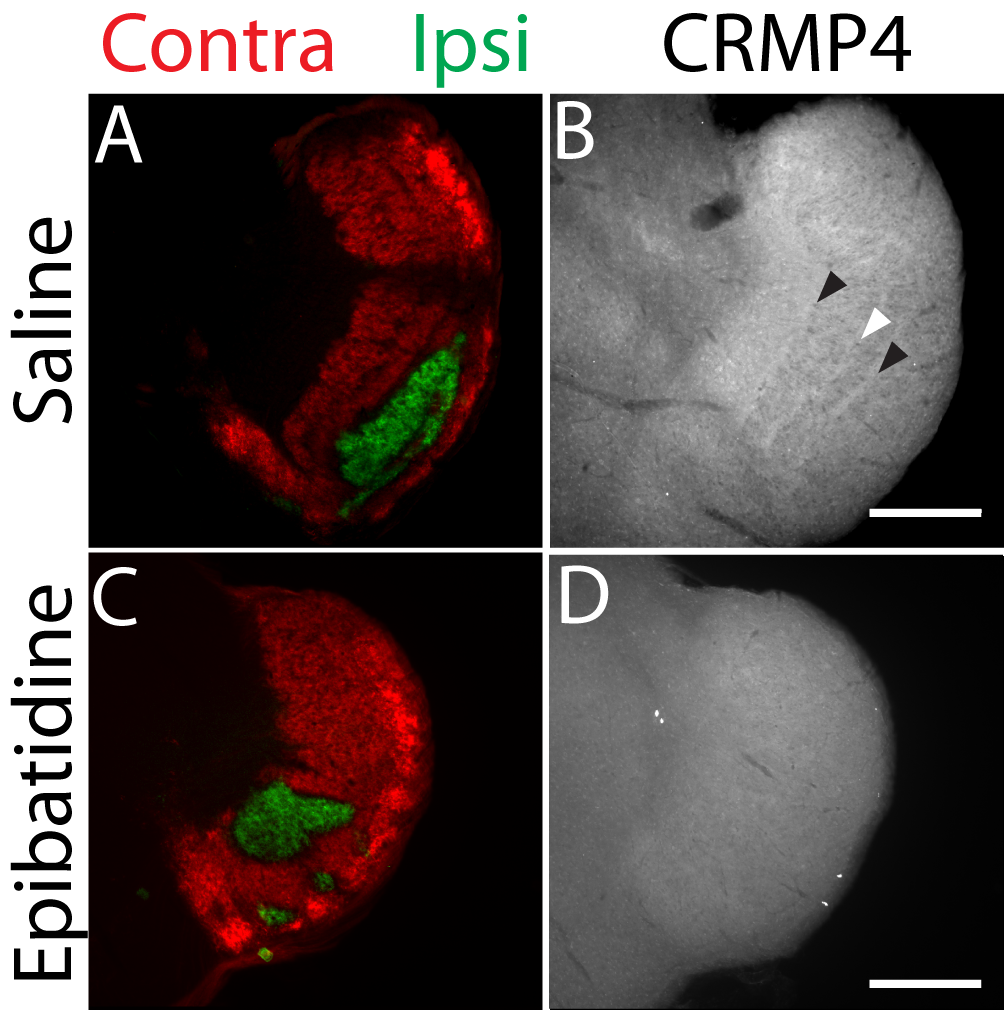
\includegraphics[width=1.0\textwidth]{FigureImages/EpiCRMP4.png}
\end{center}
\caption[Epibatidine treatment abolishes CRMP4 expression in the ferret LGN.]{Epibatidine treatment abolishes CRMP4 expression in the ferret LGN. Bilateral  intraocular treatment with epibatidine (1mM) from P1-P9 followed by recovery until P30 results in a disorganized retinothalamic projection (A, saline treated vs. C, epibatidine treated).  Epibatidine treatment abolishes normal CRMP4 expression in the nucleus (B, saline treated vs. D, epibatidine treated).  Black arrowheads indicate interlaminar zone staining and white arrowheads indicate staining at the within layer ON/OFF boundaries.  Epibatidine treated animals exhibit robust segregation of eye specific inputs to the LGN in the absence of CRMP4 expression suggesting that CRMP4 expression in the LGN is not linked to eye specific segregation. scale bars = 250$\mu$m.}
\end{figure}

\pagebreak
\begin{figure}[htb!]
\begin{center}
\leavevmode
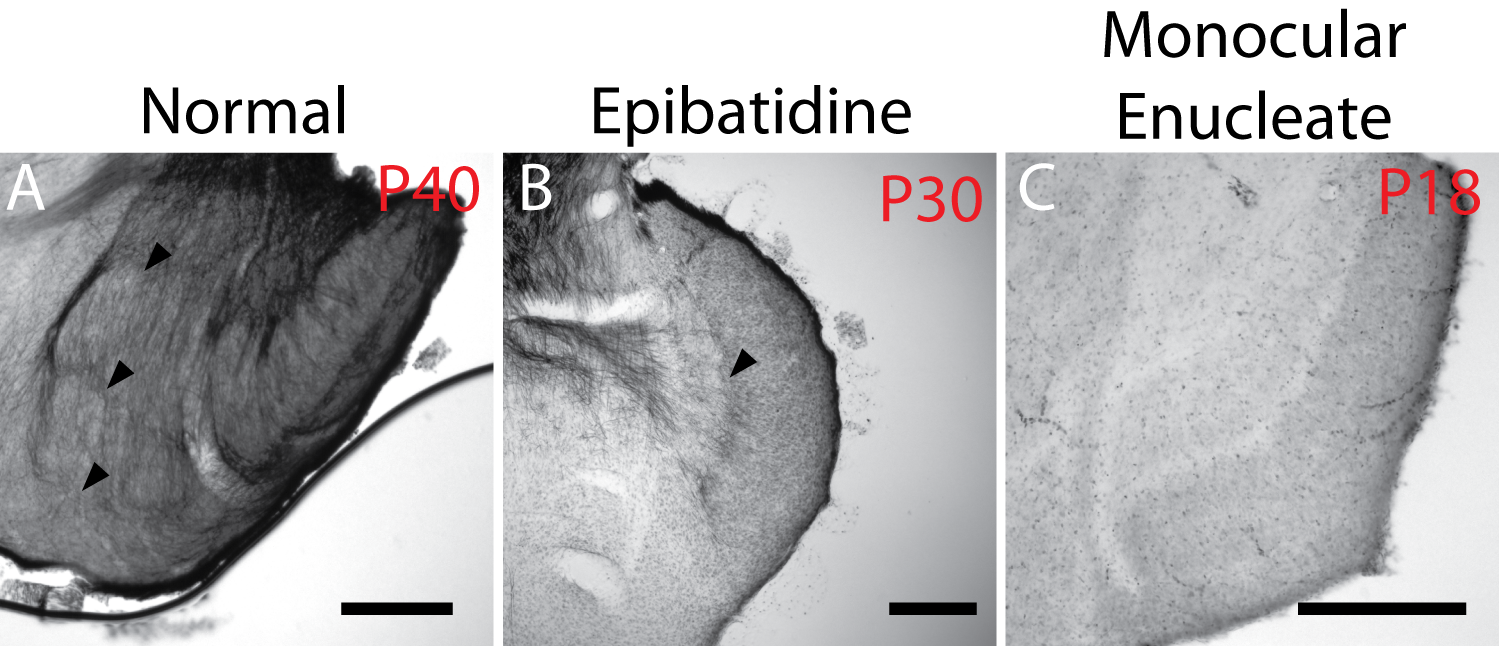
\includegraphics[width=1.0\textwidth]{FigureImages/NormalvsEpiMyelin.png}
\end{center}
\caption[Myelination of normal and epibatidine treated LGNs.]{Myelination of normal and epibatidine treated LGNs. A, In the normal LGN, the interlaminar zones are more heavily myelinated than the main layers (arrows).  B, In the epibatidine treated ferret, only the PGN/LGN boundary is heavily myelinated (arrow).  This myelination pattern mirrors the pattern of CRMP4 in the epibatidine treated LGN.  The correlation of CRMP4 expression and myelination across both normal and epibatidine treated animals is suggestive of an interaction between the two.  CRMP4 is a mediator of myelin dependent outgrowth inhibition and may be shaping boundaries in the LGN through this mechanism.  C, In the young monocular enucleate (P18), there is no evidence of heavy myelination in the LGN.  scale bars = 250$\mu$m.}
\end{figure}
\pagebreak
%------------------------------------Chapter 4 results figs 1-----------------------------------------------
\subsection{Monocular or binocular enucleation at birth abolishes normal development of cytoarchitecture in the LGN and normal interlaminar CRMP4 expression}
n chapter 3, I reported that CRMP4 is expressed in a developmentally regulated manner in the interlaminar zones of the ferret LGN.   In order to further characterize the expression of CRMP4 in the developing LGN and shed light on the source of this protein�s expression, we performed monocular and binocular P0 enucleations followed by 16 to 55 days of recovery and immunostaining against CRMP4.  Shorter post-enucleation survival times were not explored because we aimed to characterize the impact of enucleation when CRMP4 expression is the most robust. Binocular enucleation at P0 completely eliminates CRMP4 expression in the LGN at all ages tested (P20, P26, P45, P55; figure 4.7).  CRMP4 expression in the LGNs of three ferrets (P16, figure 4.7; P18 and P20, data not shown) that were monocularly enucleated at P0 resembles a less organized version of the interlaminar expression profile seen in a normal ferret at this age.� CRMP4 is expressed around the boundaries of the A1 lamina of the LGN ipsilateral to the enucleated eye, but the expression appears to be more diffuse than in normal ferrets from this age range.� Additionally, a few CRMP4 positive cell bodies can be found in the LGN.� CRMP4 expression is not present in the LGN of older monocular enucleates at P26 and P48 (figure 4.7).  From the third to fourth postnatal week in a monocular enucleate�s life, there is a loss of the normal cytoarchitectonic laminar boundaries in the LGN.  The nucleus moves from a cytoarchitectonic state indistinguishable from age matched normals to one in which there are no discernible laminar boundaries (Guillery et al., 1985).  CRMP4 expression tracks the loss of laminar boundaries during this transition period.
%------------------------------------Chapter 4 results figs 2-----------------------------------------------
\pagebreak
\begin{figure}[htb!]
\begin{center}
\leavevmode
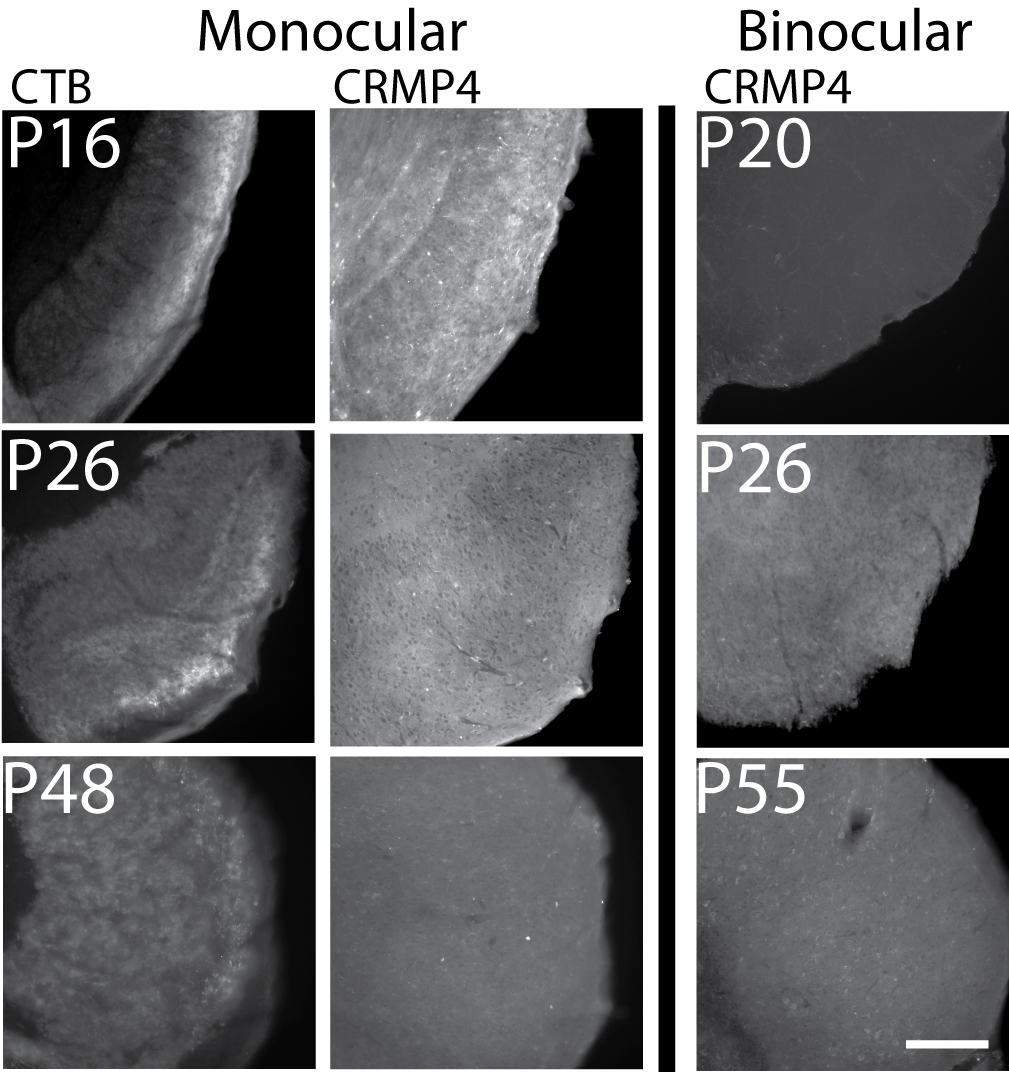
\includegraphics[width=0.8\textwidth]{FigureImages/EnucleationCRMP4.png}
\end{center}
\caption[LGN  CRMP4 expression in enucleate ferrets.]{LGN  CRMP4 expression in enucleate ferrets. GN expression of CRMP4 in ferrets enucleated at P0 and sacrificed at the ages shown.  Left column, spared contralateral retinal afferents in monocularly enucleated ferrets labeled with cholera toxin � subunit conjugated to alexa 488.  By P26, the contralateral projection has begun to fill the whole volume of the LGN with robust contralateral projections throughout the nucleus by P48.  Middle column, CRMP4 immunostaining data from the same sections as the left column, the expansion of the contralateral projection is coincident with loss of CRMP4 expression.  Right column, binocular enucleation completely abolishes laminar expression of CRMP4 at all survival periods tested as shown by immunostaining.  All sections are horizontal and 50$\mu$m thick. Scale bar =250$\mu$m, applies to all.}
\end{figure}
\pagebreak
%------------------------------------Chapter 4 results figs 2-----------------------------------------------

\section{Conclusions}
\subsection{Summary of Findings}
I confirm here that transient block of cholinergic retinal waves from P0 to P10 using epibatidine disrupts the normal projection pattern of retinal afferents into the LGN and   eliminates normal cytoarchitectural laminar boundaries.  These results are consistent with previous reports (Huberman et al., 2002; Padmanabhan, 2008).  Further, I obtain the same results using methods employed previously in our lab (Padmanabhan, 2008).     I show that epibatidine results in the loss of normal CRMP4 expression and abolishes normal myelination patterns in the LGN.  

I also show that a loss of CRMP4 expression in the LGN is observed in animals subjected to either binocular or monocular enucleation at birth.  In the binocular enucleate, CRMP4 expression appears to never develop in the LGN.  In the monocular enucleate, CRMP4 expression is initially present at P16 when CRMP4 expression normally develops.  However, CRMP4 expression is more diffuse and disorganized than in the normal animal and rapidly declines.  The decline of CRMP4 expression tracks the loss of cell sparse interlaminar zones in monocular enucleates.

\subsection{Pitfalls and limitations}
First, because of the length of time between epibatidine injections (48 hrs), it is almost certainly the case that the blockade of retinal waves is incomplete throughout the first ten days of life, but it is rather intermittent with some recovery between injections.  Intermittent recovery of this kind most likely induces variability into the final disruption of retinothalamic  targeting in epibatidine treated animals.  In spite of this, it is remarkable that epibatidine animals can be treated as a group and be distinguished from controls on some salient measures of retinothalamic morphology (i.e. number of ipsilateral patches).  A second limitation of this study is that no other retinal activity modulation paradigm was carried out.  It is not possible to know for sure if the observed reduction in CRMP4 expression in the LGN is specific to epibatidine treatment or if it is a result of modulated retinal activity in general.  However, the aim of this chapter is simply to measure the impact of altered LGN morphology on CRMP4 expression and my data is useful in that regard.

\subsection{Discussion}
In both epibatidine treated animals and enucleate animals, CRMP4 expression in the LGN appears to be linked to the cytoarchitectural landscape of the nucleus.  Specifically, CRMP4 expression tracks the presence, absence, or change in the cell sparse interlaminar zones that define the boundaries of LGN laminae in normal animals.  I reported in chapter 3 that CRMP4 expression is apparent at the interlaminar zones in the normal ferret and that CRMP4 expression is developmentally regulated.  Here, I have shown that abolishing the interlaminar zones through enucleation or blockade of cholinergic retinal waves with epibatidine also abolishes CRMP4 expression.  Further, CRMP4 expression tracks the degradation of interlaminar zones in monocular enucleates.  In these animals, normal LGN cytoarchitecture develops initially and persists into the third week of postnatal life but interlaminar zones are soon lost and the mature monocular enucleate lacks them altogether (Guillery et al., 1985).  CRMP4 expression in monocular enucleates mirrors this pattern, showing diffuse expression around the interlaminar zones during the third postnatal week and disappearing by the end of the forth postnatal week.  Taken together, these results indicate that the presence of cell sparse interlaminar zones and CRMP4 expression are at least coincidently linked.  

Myelination in the LGN also appears to be linked to the presence or absence of the cell sparse interlaminar zones.  In chapter 3, I reported that the interlaminar zones of the ferret LGN are more heavily myelinated than the rest of the nucleus. Dense myelination of this kind fails to develop in epibatidine treated animals and in enucleates.  Instead, only the medial boundary of the nucleus exhibits dense myelination.  The fact that myelination and CRMP4 expression both track the presence or absence of the cell sparse interlaminar zones suggests a possible mechanism by which CRMP4 may be sculpting the locations of retinal afferents in the LGN.  CRMP4 has been shown to be a mediator of myelin dependent neurite outgrowth inhibition (Alabed et al., 2007).  It is possible that CRMP4 expression in retinal ganglion cell afferents serves to mediate the translation of extracellular myelination cues into axon outgrowth inhibition at laminar boundaries (see general discussion for a more in depth treatment).  Under this scheme, the failure of myelination to develop in epibatidine and monocular enucleate LGNs is permissive for axonal rearrangement in the area of normal laminar boundaries.  In both cases,  retinal ganglion cell afferents cross regions that would be defined by heavily myelinated and cell sparse interlaminar zones and would normally serve as barriers to axonal outgrowth.  Myelination may also be partially required for the maintenance of CRMP4 expression.  There is no detectable laminar myelination in young monocular enucleates.  The fact that CRMP4 expression initially develops in the LGNs of these animals but does not persist lends support to the hypothesis that LGN CRMP4 expression may be maintained in part by the presence of local myelination cues.